\documentclass[../main.tex]{subfiles}

\begin{document}

\problem{2}

Consider the problem of two steady, uniform, and incompressible fluid jets colliding at right angles as shown to form a common jet at an angle \(\theta\). 
The pressure everywhere is \(p_atm\), and gravity/shear stress can be safely neglected. 
The control volume is given by the dashed lines.
Write out, simplify (stating your assumptions), and solve the continuity equation and relevant momentum equations. 
Find the angle \(\theta\) in terms of the flow properties \(u_1, \dot{m}_1, v_2, \ \textrm{and} \ \dot{m}_2\) of the two jets (where \(\dot{m}\) is the mass flowrate). 
State your assumptions.

\begin{figure}[ht]
    \centering
    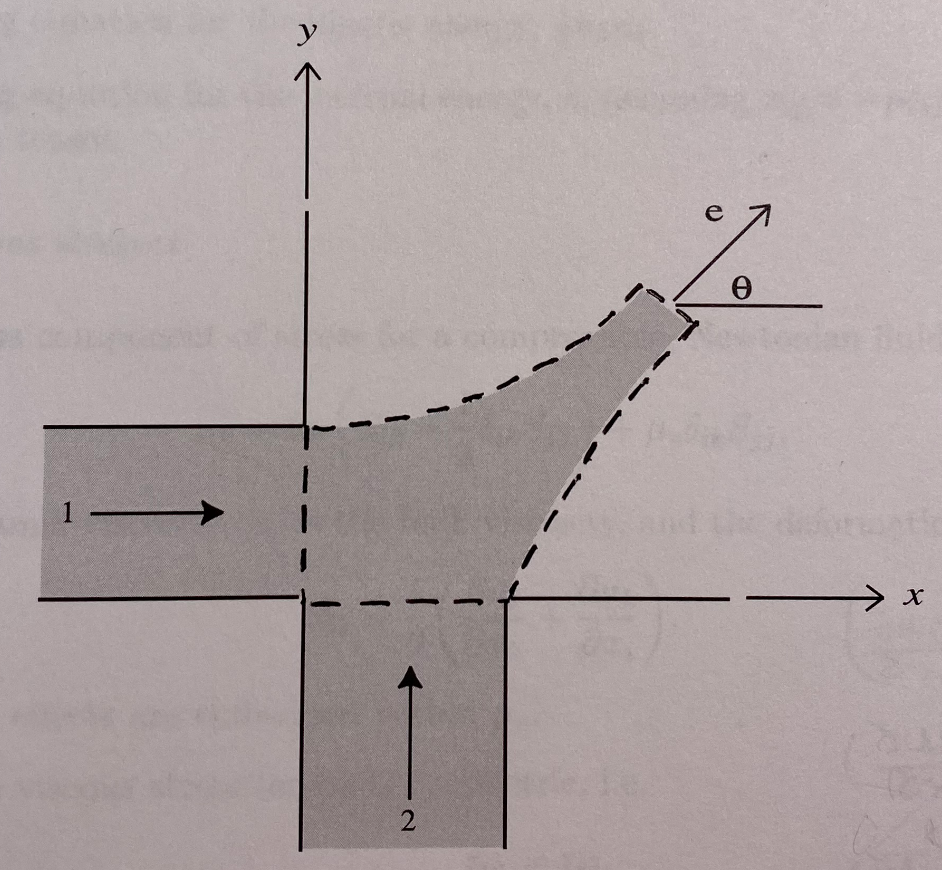
\includegraphics[scale=0.5]{images/problem2_diagram.png}
\end{figure}

\givens{}
Something

\assumptions{}
Something else

\solution{}
Yet again, more

\end{document}